\subsection{Pix2Pix-Kernkonzepte}
\subsubsection{Generator}
Die Bildverarbeitung hat in den letzten Jahren durch den Einsatz tiefer neuronaler Netzwerke erhebliche Fortschritte gemacht. Im Mittelpunkt vieler dieser Fortschritte steht die U-Net-Architektur, die speziell für die Bildsegmentierung entwickelt wurde. Diese Architektur zeichnet sich durch ihre angeklügelte Kombination aus Encoder- und Decoder- Strukturen sowie durch den Einsatz von Skip-Verbindungen aus.
 \newline
Bei der Encoder-Decoder-Struktur handelt es sich um einen Ansatz, bei dem das Eingangsbild zunächst durch den Encoder schrittweise reduziert wird. Dieser Prozess dient dazu, wesentliche Merkmale des Bildes zu erfassen. Anschließend wird das Bild durch den Decoder wiederhergestellt, indem die zuvor extrahierten Merkmale verwendet werden. Während dieser Prozesse besteht jedoch das Risiko des Informationsverlustes, insbesondere in den tieferen Schichten des Netzwerks.
Um dieses Problem zu adressieren, führt die U-Net-Architektur Skip-Verbindungen ein. Diese direkten Verbindungen zwischen korrespondierenden Schichten des Encoders und Decoders sorgen dafür, dass Detailinformationen nicht verloren gehen. Genauer gesagt, ermöglichen diese Verbindungen den direkten Informationsfluss zwischen jeweils äquivalenten Schichten, wodurch die Rekonstruktion des Bildes im Decoder mit einer höheren Genauigkeit erfolgt. \newline
Die Bedeutung von Skip-Verbindungen zeigt sich insbesondere in Anwendungen wie der Bild-zu-Bild-Übersetzung. Hier muss oft ein Bild mit niedriger Auflösung in ein Bild mit hoher Auflösung überführt werden, ohne dass Details verloren gehen. Die U-Net-Architektur, die angereichert mit diesen Verbindungen ist, ermöglicht daher eine feinere Rekonstruktion, die sowohl globale als auch lokale Informationen berücksichtigt. \newline
Somit kann die U-Net-Architektur durch ihre Kombination aus Encoder-Decoder-Struktur und Skip-Verbindungen ein effektives Werkzeug für die Bildsegemtierung darstellen. Ihre Fähigkeit, sowohl globale Muster als auch feine Details zu berücksichtigen, macht sie zu einer bevorzugten Wahl für viele Bildverarbeitungsaufgaben. \newline
In Abbildung \ref{fig:unet} ist die typische U-Net-Architektur dargestellt. Die linke Seite des ''U'' repräsentiert den Encoder-Teil, der das Eingangsbild schrittweise reduziert und wesentliche Merkmale extrahiert. Die rechte Seite repräsentiert den Decoder-Teil, der das Bild mithilfe der extrahierten Merkmale rekonstruiert. Die horizontalen Linien repräsentieren die Skip-Verbindungen, die sicherstellen, dass Detailinformationen zwischen den korrespondierenden Schichten des Encoder und Decoders direkt übertragen werden. \newline 
In der Pix2Pix Technologie dient diese U-Net-Architektur als Generator. Er ist das zentrale Element, das für die Bild-zu-Bild-Übersetzung verantwortlich ist. Die Wahl der U-Net-Struktur für den Generator liegt in ihrer Fähigkeit, feinere Details und Kontextinformationen aus dem Eingangsbild beizubehalten, was für die Bild-zu-Bild-Übersetzung von entscheidender Bedeutung ist. Die Encoder-Decoder-Struktur des U-Net ermöglicht es dem Generator, den globalen Kontext des Bildes zu erfassen, während die Skip-Verbindungen sicherstelle, dass auch lokale Details im resultierenden Bild berücksichtigt werden.

\begin{figure}[h]
	\centering
	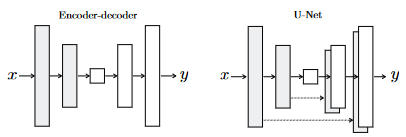
\includegraphics[width=0.7\linewidth]{./images/unet.png}
	\caption{Schematische Darstellung der U-Net-Architektur. Die Architektur besteht aus einem Encoder-Teil (links), einem Decoder-Teil (rechts) und Skip-Verbindungen zwischen korrespondierenden Schichten.}
	\label{fig:unet}
\end{figure}

\subsubsection{Diskriminator}

Im adversariellen Lernprozess spielen Generatoren und Diskriminatoren eine entscheidende Rolle. Während der Generator versucht, Daten zu erzeugen, die von echten Daten kaum zu unterscheiden sind, evaluiert der Diskriminator die vom Generator erzeugten Daten und versucht, zwischen echten und gefälschten Daten zu unterscheiden.\newline
Im Kontext von Generative Adverserial Networks (GANs), insbesondere im speziellen Fall des Pix2Pix GANs, spielt der PatchGAN-Diskriminator eine besonders wichtige Rolle. Der zentrale Unterschied dieses Diskriminators zu traditionellen Diskriminatoren liegt in der Art und Weise, wie er Bilder bewertet. Statt das gesamte Bild zu beurteilen, zerlegt der PatchGAN-Diskriminator das Bild in mehrere kleinere Bildabschnitte oder Patches und bewertet jeden Patch einzeln auf seine Echtheit. \newline
Ein solches Vorgehen hat den klaren Vorteil, dass feinere Strukturen und Details in den Bildern erkannt und beurteilt werden können. Durch diese segmentierte Beurteilung kann der Diskriminator besser einschätzen, ob die Struktur und Beschaffenheit eines bestimmten Bildteils realistisch ist. Dies ist besonders nützlich, da kleinere Unstimmigkeiten in den Bildern, die ein traditioneller Diskriminator möglicherweise übersieht, vom PatchGAN erfasst werden können. \newline
Ein weiterer Vorteil des PatchGAN-Diskriminators ist seine Skalierbarkeit. Da er auf festen Patchgrößen basiert, kann er flexibel auf Bilder unterschiedlicher Größen angewendet werden, ohne dass das zugrunde liegende Modell geändert werden muss. Dies führt nicht nur zu einer schnelleren Bildverarbeitung, sondern ermöglicht auch eine effiziente Ausführung auf großen Bildern. Darüber hinaus reduziert es potenzielle Kachelartefakte, die bei traditionellen Diskriminatoren auftreten können.\newline
Eine Metrik, die oft verwendet wird, um die Leistung des Diskriminator zu beurteilen, ist der FCN-Score. Dieser bewertet die Qualität der vom Generator erzeugten Bilder. Ein hoher FCN-Score zeigt, dass der Diskriminator erfolgreich echte von gefälschten Bildern unterscheiden kann. \newline
Der PatchGAN-Diskriminator kann wenn er effektiv eingesetzt wird, zu besseren und realistischeren Bildern im adverseriellen Lernprozess beitragen. Seine Fähigkeit, lokale Bildinformationen zu bewerten, ermöglicht es auch subtile Unterschiede in den Bildern zu erkennen, was zu einer verbesserten Qualität der generierten Bilder führt.